The GERmanium Detector Array (GERDA) experiment \cite{Abt:2004yk}, located in Hall A of the Laboratori Nazionali del Gran Sasso (LNGS), will make use of naked Ge detectors immersed in a large cryostat of ultra-pure LAr.

The Ge detectors are organized in strings (2--5 detectors) and mounted in special low-mass ($\sim 80$ g) holders made of ultra-pure copper and PTFE. The array of strings is contained in a vacuum insulated stainless steel cryostat of 4.2 m diameter and 8.9 m height. A copper shield covers the inner cylindrical shell of the cryostat with a maximum thickness of 6 cm. The cryostat is placed in a water tank, of 10 m diameter and 9.4 m height, serving as a gamma and neutron shield. It will be also used as a veto against cosmic rays thanks to its instrumentation with 66 photomultipliers, with good efficiency in detecting the Cherenkov light. The cosmic muon veto is reinforced by plastic scintillator panels on top of the detector, for a surface of about 20 m$^2$. A drawing of the detector and shielding is shown in fig.~\ref{fig:gerda}.

%%%%%
\begin{figure}[t!]
\begin{center}
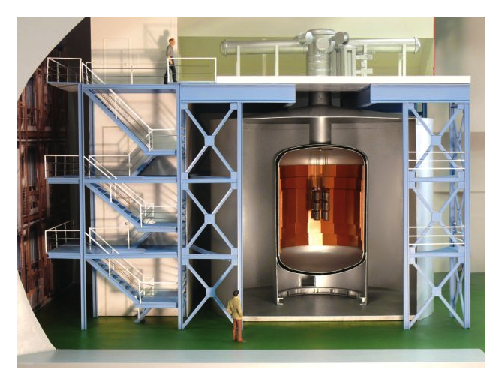
\includegraphics[]{img/gerda.eps}
\end{center}
\caption{Sketch of the GERDA experiment. The germanium arrays can be seen inside the copper cryostat, and this one placed inside the cylindrical water tank.} \label{fig:gerda}
\end{figure}
%%%%%

In its first phase, GERDA-1, eight fully refurbished germanium diodes (17.7 kg total active mass, 86\% isotopic enrichment in \GE ) from the previous Heidelberg-Moscow and IGEX experiments will be used. In the subsequent step, GERDA-2, new diodes will be used for a total active mass of 35.4 kg. These new diodes will be p-type Broad Energy (BEGe) detectors \cite{Budjas:2008wb,Agostini:2010ke}, allowing for a better discrimination of backgrounds thanks to a sophisticated pulse shape discrimination.

The experiment started commissioning runs in June 2010 using natural Ge, low-background, detectors, refurbished from the Genius-TF experiment. These commissioning runs focused on the investigation of the background sources (most notably on the unexpectedly large contribution from $^{42}$Ar-$^{42}$K in the LAr) and on $^{42}$Ar background mitigation strategies, see sect.~\ref{subsec:sensi_assumptions}. Data taking for the GERDA-1 physics run will start in the next months. The background level of the natural Ge setup was measured to be $0.06\pm 0.02$ \ckky\ (corresponding to $0.07\pm 0.02$ \ckkbby ), consistent with early indications from the first string of enriched Ge detectors deployed \cite{Cattadori:2012fy}. This rate, obtained without using pulse shape information, is a factor of 3--4 lower than the HM and IGEX measured ones (see sect.~\ref{subsec:past}), but still about a factor of 6 higher than the GERDA-1 goal. The reason for this higher than expected background rate is at present not fully understood. The goals of GERDA-2 are to start data taking in about two years, with about twice the isotope mass of GERDA-1, and with a background level of 0.001 \ckky\ (or 0.0012 \ckkbby ).

In the very long term a third phase of the experiment, GERDA-3, is foreseen to make use of about 1 ton of $^{76}$Ge target material together with a further reduction of background. Such an effort, common with the MAJORANA project (see below), would be feasible only in a word-wide collaboration, and provided that the GERDA approach could demonstrate to be the best candidate technology to push the double beta decay sensitivity below the inverted hierarchy mass threshold (about 30 meV). 
